\documentclass[11pt,a4paper]{article}
\usepackage[margin=2.6cm]{geometry}
\usepackage[T1]{fontenc}
\usepackage[utf8]{inputenc}
\usepackage{lmodern}
\usepackage{amsmath,amssymb,amsthm,bm}
\usepackage{booktabs}
\usepackage{graphicx}
\usepackage{microtype}
\usepackage[hidelinks]{hyperref}
\usepackage{enumitem}
\setlist{nosep}
\newcommand{\R}{\mathbb{R}}
\newcommand{\CE}{\mathrm{CE}}
\newcommand{\RCE}{\mathrm{RobustCE}}
\newcommand{\UU}{\mathcal{U}_{\Delta}}
\title{Cross-Entropy versus Robust Cross-Entropy\\under Uncertainty in Target Distributions}
\author{Student name: \textit{Andrej Mymrin}}
\date{\today}
\begin{document}
\maketitle

\section{Formulation and mathematical analysis}
For a $K$-class classification problem, let $p\in\Delta_K$ denote the predicted
probability vector, with $p_j>0$, and let $\mu\in\Delta_K$ be the nominal target,
where
\begin{equation}
    \Delta_K=\bigl\{c\in\R^K:c_j\geq 0,\ \bm{1}^{\mathsf T}c=1\bigr\}.
\end{equation}
The nominal cross-entropy loss is
\begin{equation}
    \ell_{\CE}(p;\mu)=-\mu^{\mathsf T}\log p.
\end{equation}
Given a positive-definite matrix $\Sigma$ and an uncertainty radius $\rho\geq 0$,
the target uncertainty set and robust cross-entropy are
\begin{align}
    \UU(\mu,\Sigma,\rho)
      &=\left\{c\in\Delta_K:(c-\mu)^{\mathsf T}\Sigma^{-1}(c-\mu)
                  \leq\rho^2\right\},\\
    \ell_{\RCE}(p;\mu,\Sigma,\rho)
      &=\max_{c\in\UU(\mu,\Sigma,\rho)}-c^{\mathsf T}\log p.
\end{align}
The matrix $\Sigma$ describes the geometry of uncertainty in the \emph{target
distribution}; it is not a gradient covariance matrix. We analyze this objective
before considering model training.

\subsection*{(a) Simplex constraints and the unconstrained support function}
The simplex constraints $c_j\geq 0$ and $\bm{1}^{\mathsf T}c=1$ ensure that
$c$ is a probability distribution. Without them, the ellipsoid may include
negative components or vectors whose entries do not sum to one, neither of
which represents a meaningful class target.

To derive the expression without these constraints, write $g=-\log p$ and
consider
\begin{equation}
    \max_{(c-\mu)^{\mathsf T}\Sigma^{-1}(c-\mu)\leq\rho^2}
    g^{\mathsf T}c.
\end{equation}
Set $c=\mu+\Sigma^{1/2}u$. The constraint becomes $\lVert u\rVert_2\leq\rho$,
so Cauchy--Schwarz gives
\begin{align}
    \max_{\lVert u\rVert_2\leq\rho}
    \left(g^{\mathsf T}\mu+(\Sigma^{1/2}g)^{\mathsf T}u\right)
      &=g^{\mathsf T}\mu+\rho\lVert\Sigma^{1/2}g\rVert_2\\
      &=-\mu^{\mathsf T}\log p
          +\rho\sqrt{(\log p)^{\mathsf T}\Sigma(\log p)}.
\end{align}
For $\rho>0$, one unconstrained maximizer is
\begin{equation}
    c_{\mathrm{ell}}^*
      =\mu-\rho\frac{\Sigma\log p}
                   {\sqrt{(\log p)^{\mathsf T}\Sigma(\log p)}}.
\end{equation}
The denominator is nonzero because all components of a strictly positive
probability vector cannot equal one simultaneously when $K\geq2$.
The ellipsoid contains $\UU$, and thus
\begin{equation}
    \ell_{\RCE}(p;\mu,\Sigma,\rho)
    \leq -\mu^{\mathsf T}\log p
          +\rho\sqrt{(\log p)^{\mathsf T}\Sigma(\log p)}.
\end{equation}
The right-hand side is generally only an upper bound: the unconstrained
maximizer need not lie in $\Delta_K$. It equals the simplex-constrained maximum
only when an unconstrained maximizer is feasible for the simplex as well.

\subsection*{(b) Zero radius, lower bound, and monotonicity}
Since $\Sigma^{-1}$ is positive definite,
\begin{equation}
    (c-\mu)^{\mathsf T}\Sigma^{-1}(c-\mu)=0
    \quad\Longleftrightarrow\quad c=\mu.
\end{equation}
At $\rho=0$, therefore, $\UU(\mu,\Sigma,0)=\{\mu\}$, and
\begin{equation}
    \boxed{\ell_{\RCE}(p;\mu,\Sigma,0)=\ell_{\CE}(p;\mu).}
\end{equation}
For any $\rho\geq0$, the nominal target $\mu$ is feasible. Maximizing over a
set containing $\mu$ gives the lower bound
\begin{equation}
    \boxed{\ell_{\RCE}(p;\mu,\Sigma,\rho)\geq\ell_{\CE}(p;\mu).}
\end{equation}
Finally, if $0\leq\rho_1\leq\rho_2$, then
$\UU(\mu,\Sigma,\rho_1)\subseteq\UU(\mu,\Sigma,\rho_2)$, hence
\begin{equation}
    \ell_{\RCE}(p;\mu,\Sigma,\rho_1)
    \leq\ell_{\RCE}(p;\mu,\Sigma,\rho_2).
\end{equation}
Thus the robust loss is nondecreasing in the radius \emph{at a fixed prediction}.
The increase may be zero, particularly after the set has expanded to include
all simplex targets. This statement does not imply that a model trained with a
larger radius must have a larger test loss: its learned predictions may change.

\subsection*{(c) Binary formulation and worst-case target}
Use the ordering specified in the assignment:
\begin{equation}
    p=(1-p_1,p_1)^{\mathsf T},\qquad
    \mu=(1-m,m)^{\mathsf T},\qquad
    c=(1-q,q)^{\mathsf T},\qquad
    \Sigma=\tau^2 I_2,\quad\tau>0.
\end{equation}
Here $p_1$ and $q$ are the predicted and target probabilities of class 1.
The ellipsoidal condition reduces to
\begin{align}
    (c-\mu)^{\mathsf T}\Sigma^{-1}(c-\mu)
      &=\frac{(m-q)^2+(q-m)^2}{\tau^2}
       =\frac{2(q-m)^2}{\tau^2}\leq\rho^2.
\end{align}
Defining the effective radius
\begin{equation}
    \boxed{\delta=\frac{\rho\tau}{\sqrt{2}}},
\end{equation}
we obtain $|q-m|\leq\delta$. Intersecting with $0\leq q\leq1$ gives
\begin{equation}
    \boxed{q\in[q_L,q_U],\qquad
       q_L=\max\{0,m-\delta\},\quad q_U=\min\{1,m+\delta\}.}
\end{equation}
For a fixed prediction, cross-entropy as a function of $q$ is
\begin{equation}
    L(q;p_1)=-(1-q)\log(1-p_1)-q\log p_1
            =-\log(1-p_1)+q\log\frac{1-p_1}{p_1}.
\end{equation}
It is affine in $q$, with slope
$\partial L/\partial q=\log((1-p_1)/p_1)$. The maximizing endpoint is therefore
\begin{equation}
    q^*(p_1)=
    \begin{cases}
      q_U, & p_1<\tfrac12,\\
      \text{any }q\in[q_L,q_U], & p_1=\tfrac12,\\
      q_L, & p_1>\tfrac12.
    \end{cases}
\end{equation}
Substitution gives the explicit robust loss
\begin{equation}
    \boxed{\ell_{\RCE}(p_1;m,\delta)=
    \begin{cases}
    -(1-q_U)\log(1-p_1)-q_U\log p_1,&p_1<\tfrac12,\\
    \log2,&p_1=\tfrac12,\\
    -(1-q_L)\log(1-p_1)-q_L\log p_1,&p_1>\tfrac12.
    \end{cases}}
\end{equation}
The corresponding worst-case target vector is
$c^*=(1-q^*,q^*)^{\mathsf T}$. The case $p_1=1/2$ is a tie: all feasible targets
give the same loss, although the value itself remains well defined.

Only the product $\rho\tau$ enters the binary interval, through $\delta$.
Consequently, pairs $(\rho,\tau)$ with the same product define identical
binary uncertainty sets and identical robust losses; varying them separately
at fixed product does not generate a new binary model.

\subsection*{(d) Numerical example for an observed label $y=0$}
For an observed binary label, set $m=y$. With $y=0$ and $\delta=0.2$,
\begin{equation}
    q_L=0,\qquad q_U=0.2,\qquad
    \ell_{\CE}(p;0)=-\log(1-p_1).
\end{equation}
We use natural logarithms throughout. For $(0.9,0.1)$ and $(0.6,0.4)$,
$p_1<1/2$, so $q^*=0.2$ and $c^*=(0.8,0.2)^{\mathsf T}$. For $(0.4,0.6)$,
$p_1>1/2$, so $q^*=0$ and $c^*=(1,0)^{\mathsf T}$. The losses are
\begin{align}
    p=(0.9,0.1):\quad &\ell_{\CE}=-\log0.9\approx0.1054,\\
    &\ell_{\RCE}=-0.8\log0.9-0.2\log0.1\approx0.5448;\\[2pt]
    p=(0.6,0.4):\quad &\ell_{\CE}=-\log0.6\approx0.5108,\\
    &\ell_{\RCE}=-0.8\log0.6-0.2\log0.4\approx0.5919;\\[2pt]
    p=(0.4,0.6):\quad &\ell_{\CE}=-\log0.4\approx0.9163,\\
    &\ell_{\RCE}=-\log0.4\approx0.9163.
\end{align}
\begin{table}[htbp]
\centering
\caption{Nominal and robust cross-entropy for $y=0$ and $\delta=0.2$.}
\begin{tabular}{@{}cccc@{}}
\toprule
Prediction $p$ & CE & RobustCE & Worst-case target $c^*$\\
\midrule
$(0.9,0.1)$ & 0.1054 & 0.5448 & $(0.8,0.2)$\\
$(0.6,0.4)$ & 0.5108 & 0.5919 & $(0.8,0.2)$\\
$(0.4,0.6)$ & 0.9163 & 0.9163 & $(1.0,0.0)$\\
\bottomrule
\end{tabular}
\end{table}

For the two correct predictions, the worst-case target transfers some mass to
class 1, which the model regards as less likely. This increases the robust loss,
particularly for the confident prediction $(0.9,0.1)$. In contrast, the
misclassified prediction $(0.4,0.6)$ receives no additional penalty: the
nominal one-hot target already maximizes the loss on the feasible interval.
The worst-case construction can therefore discourage extreme confidence, but
it does not automatically protect against incorrect observed training labels.
A corrupted label is still treated as the center of the target uncertainty set.

\subsection*{(e) Convexity in predictions and model parameters}
For any fixed $c\in\Delta_K$, define
$f_c(p)=-\sum_{j=1}^K c_j\log p_j$ on the positive simplex. Its Hessian is
\begin{equation}
    \nabla_p^2 f_c(p)
    =\operatorname{diag}\!\left(\frac{c_1}{p_1^2},\ldots,
                                     \frac{c_K}{p_K^2}\right)\succeq0.
\end{equation}
Thus $f_c$ is convex in $p$. Taking $c=\mu$ proves convexity of nominal
CE. RobustCE is the pointwise maximum of these convex functions over the fixed
uncertainty set $\UU$, so it is also convex in $p$. The maximum need not be
differentiable where the worst-case target changes.

Convexity in predictions does not by itself establish convexity in model
parameters. For binary logistic regression, however, let
\begin{equation}
    s_\theta(a)=w^{\mathsf T}a+b,\qquad p_1=\sigma(s_\theta(a)),
    \qquad\sigma(s)=\frac{1}{1+e^{-s}}.
\end{equation}
For each fixed target probability $q$, the loss is
\begin{equation}
    L(s;q)=\log(1+e^s)-qs,
    \qquad \frac{\partial^2 L}{\partial s^2}
            =\sigma(s)\bigl(1-\sigma(s)\bigr)>0.
\end{equation}
It is convex in $s$, and $s_\theta$ is affine in $\theta=(w,b)$. Hence nominal
CE is convex in the logistic-regression parameters. The robust loss can be
written as $\max_{q\in[q_L,q_U]}L(s_\theta;q)$, a pointwise maximum of convex
functions of $\theta$; it is therefore convex too. Averaging over training
examples preserves this property. Convexity does not, however, guarantee a
unique minimizer.

For a nonlinear network, such as
\begin{equation}
    s_\theta(a)=w_2^{\mathsf T}\tanh(W_1a+b_1)+b_2,
\end{equation}
logits are no longer affine in the network parameters. Composing either loss
with this nonlinear parameterization generally yields a nonconvex training
objective. Therefore, the convexity result for logistic regression cannot be
extended to the two-layer network; gradient-based training is not generally
guaranteed to find a global optimum.

\section{Implementation and checks}
The NumPy implementation works with the class-1 logit $s$, so that
$p_1=\sigma(s)$. For any class-1 target mass $q$, it evaluates
\begin{equation}
    L(s;q)=(1-q)\operatorname{softplus}(s)+q\operatorname{softplus}(-s),
    \qquad \operatorname{softplus}(s)=\operatorname{logaddexp}(0,s).
\end{equation}
This form avoids taking the logarithm of rounded probabilities and avoids
subtracting two large, nearly equal terms for confident correct predictions.
CE uses $q=m$. RobustCE takes $q=q_U$ for $s<0$ and $q=q_L$ for $s>0$,
with endpoints computed using $\delta=\rho\tau/\sqrt{2}$. The selected
branch gives logit derivative $\sigma(s)-q^*$. At $s=0$ the set of
subgradients in the logit is $[1/2-q_U,1/2-q_L]$. The code chooses $q^*=m$
at this tie, giving the valid subgradient $1/2-m$. It propagates these
per-example derivatives through each model, averages them and uses Adam to
update the model parameters.

\subsection*{(a) Numerical checks}
The script \texttt{checks.py} reproduces the CE and RobustCE values in
Section~1(d), including the active target. Across 2,051 logits, including
$-1000$, $0$ and $1000$, it checks exact equality at zero radius, finiteness,
and the nominal lower bound through successive radii up to full saturation.
At $\delta=1$ it also checks that the loss equals
$\operatorname{softplus}(|s|)$. An independent direct search evaluates
probability-space CE at 2,001 evenly spaced targets, including both feasible
endpoints, for each of 175 combinations of prediction, nominal target and
radius. The largest absolute discrepancy with the analytic loss was
$8.88\times10^{-16}$. Central finite differences checked the derivative away
from ties, and the selected tie subgradient was checked against its interval.

\subsection*{(b) Label smoothing}
For an observed label $y$, we use the fixed class-1 target
$m_\varepsilon=(1-\varepsilon)y+\varepsilon/2$ in ordinary CE. This moves
$\varepsilon/2$ of the target mass to the other class, independently of the
prediction. For a correctly signed logit, RobustCE likewise moves mass away
from the observed class, by $\delta$. For an incorrectly signed logit, its
worst-case target is the observed label itself and its gradient agrees with
ordinary CE. The smoothing gradient still uses the softened target in that
case. We tune smoothing in both simulations with the clean validation procedure
in Section~\ref{sec:comparison}.

\section{Required simulations}
\label{sec:simulations}
Each seed generates independently sampled, exactly balanced training,
validation and test sets with 512, 512 and 2,048 observations, respectively.
The small training sets keep the grid search practical and leave meaningful
sampling variation across runs. The larger test sets reduce variation from
test sampling. Both problems use the generated coordinates directly. All
methods within a replicate start from identical Glorot-uniform weights and
zero biases.

\subsection{Overlapping Gaussian classes}
The first experiment draws
$a\mid y\sim\mathcal N((2y-1)(1,1)^{\mathsf T},I_2)$ and fits
$s_\theta(a)=w^{\mathsf T}a+b$. The Bayes log-odds under the balanced design
are $2(a_1+a_2)$, so the model can represent the true conditional
probability. The class overlap creates a distinction between finding the
decision boundary and estimating probabilities confidently. The probability
surfaces and $p_1=1/2$ contours are shown in Figure~\ref{fig:gaussian}.
For seed 201, the clean RobustCE and smoothing boundaries are close to
the Bayes line. CE gives a shallower line in that replicate. At 30\%
flips, the three lines are similar and the probability transitions are
more gradual, particularly for RobustCE.

\subsection{Noisy semicircles}
The second experiment draws $t\sim\operatorname{Uniform}[0,\pi]$ and
$e\sim\mathcal N(0,0.1^2I_2)$ independently, using
\begin{equation}
    a=\begin{cases}
        (\cos t,\sin t)^{\mathsf T}+e, & y=0,\\
        (1-\cos t,\tfrac12-\sin t)^{\mathsf T}+e, & y=1.
      \end{cases}
\end{equation}
It fits the width-eight tanh network from Section~1(e), with 33 parameters
shared in architecture across methods. The hidden layer allows curved
boundaries while keeping each fit inexpensive.
Figure~\ref{fig:semicircles} shows how the fitted nonlinear decision
boundary and probability surface change with label noise. With clean
labels, all three contours follow the gap between the two arcs on seed
201. RobustCE and smoothing produce less extreme probabilities. At
30\% flips, the RobustCE contour bends back in the upper-right region,
where the plotted test points are sparse. This panel illustrates one
fit, and the performance comparison uses all ten seeds.

\subsection{Training-label corruption}
For each seed, draw $u_i$ independently and uniformly on $[0,1]$ for
each training example. We test flip probabilities $\eta$ of 0, 0.15 and 0.30.
The observed training label flips when $u_i<\eta$. Every method uses the
same mask at a given rate, and higher rates retain the flips from lower
rates. We use the observed label to form the CE, RobustCE and smoothing
targets. All validation and test labels remain clean.

\section{Comparison, tuning and required outputs}
\label{sec:comparison}
\subsection{Training and clean validation selection}
Each method uses 300 full-batch Adam updates (batch size 512, moment
coefficients $0.9$ and $0.999$, numerical constant $10^{-8}$), with cosine
decay from its initial learning rate to one percent of that rate. This
budget gives a common fixed endpoint and the lower terminal rate reduces
oscillation near RobustCE's kink. Every method searches initial rates
0.001, 0.003, 0.01, 0.03, 0.10, 0.30, 0.60, 0.90, 1.20 and 1.80. RobustCE also searches
training radii $\delta$ of 0, 0.02, 0.05, 0.10, 0.20, 0.35, 0.50, 0.75 and 1.
Smoothing
uses the same numerical grid for $\varepsilon$. The strength grids cover
the full domain, with extra resolution near zero to detect modest effects.
In the initial grid, semicircle smoothing selected the largest rate, 0.60.
We added rates 0.90, 1.20 and 1.80 for every method in both simulations
and repeated the clean validation selection.

We select the smallest mean final validation RobustCE across five clean
training replicates (seeds 101--105), always evaluated at
$\delta_{\rm eval}=0.10$ with clean one-hot labels. We fixed this radius
before test evaluation to measure probability quality under a modest
worst-case shift of the clean targets. It is a modeling choice. All three
test metrics are reported so that the consequences of selection by this
criterion can be assessed. Ties are broken by smaller strength, then
smaller learning rate. The selected settings in Table~\ref{tab:settings}
are frozen for all evaluation seeds and corruption levels. We evaluate
only the final iterate. Figure~\ref{fig:radius} profiles the best learning
rate at each radius by the same validation rule.

\begin{table}[htbp]
\centering
\caption{Hyperparameters selected on the clean tuning runs. Strength denotes
$\delta$ for RobustCE and $\varepsilon$ for smoothing.}
\label{tab:settings}
\begin{tabular}{@{}llrr@{}}
\toprule
Simulation & Method & Initial rate & $\delta$ or $\varepsilon$ \\
\midrule
Gaussian & CE & 0.01 & -- \\
Gaussian & RobustCE & 0.03 & 0.1 \\
Gaussian & Smoothing & 0.03 & 0.2 \\
\addlinespace
Semicircles & CE & 0.03 & -- \\
Semicircles & RobustCE & 0.3 & 0.1 \\
Semicircles & Smoothing & 0.6 & 0.2 \\
\bottomrule
\end{tabular}

\end{table}

\subsection{Evaluation and variability}
The ten held-out seeds 201--210 vary both the sampled datasets and initial
weights, with independent random streams for the splits, initialization and
label flips. Each final model is scored on the clean test split using
accuracy with threshold $p_1\geq1/2$, ordinary CE, and RobustCE at the
common $\delta_{\rm eval}=0.10$. We also record mean predicted confidence
$\operatorname{mean}(\max(p_1,1-p_1))$ and CPU training time, excluding data
generation and metric evaluation. Tables~\ref{tab:test} and
\ref{tab:paired} give means and sample standard deviations and paired
differences between methods, respectively. Paired intervals are marginal 95\%
$t$ intervals across seeds, interpreted descriptively without multiplicity
adjustments. Plot bands are one sample standard deviation across seeds.
Figure~\ref{fig:learning} plots common clean validation CE during
optimization, and Figure~\ref{fig:corruption} uses the held-out test metrics.
On clean data the tuned RobustCE and smoothing runs reach their
validation CE plateaus sooner than CE. At 30\% flips on semicircles,
CE reaches the lowest final validation CE of the three. The learning
curves reflect the separately tuned learning rates and the objectives.

\begin{table}[p]
\centering
\small
\caption{Clean test performance and training wall time over ten seeds
(mean $\pm$ sample SD). RobustCE uses the fixed evaluation radius $0.10$.
Conf. denotes mean predicted confidence.}
\label{tab:test}
\resizebox{\textwidth}{!}{\begin{tabular}{@{}lrlrrrrr@{}}
\toprule
Simulation & $\eta$ & Method & Acc. (\%) & CE & RobustCE & Conf. & Time (s) \\
\midrule
Gaussian & 0.00 & CE & $89.56\pm3.54$ & $0.325\pm0.122$ & $0.490\pm0.056$ & $0.783\pm0.098$ & $0.040\pm0.011$ \\
Gaussian & 0.00 & RobustCE & $91.98\pm0.90$ & $0.277\pm0.010$ & $0.439\pm0.006$ & $0.801\pm0.007$ & $0.048\pm0.009$ \\
Gaussian & 0.00 & Smoothing & $91.99\pm0.90$ & $0.274\pm0.010$ & $0.439\pm0.006$ & $0.804\pm0.006$ & $0.036\pm0.007$ \\
\addlinespace
Gaussian & 0.15 & CE & $89.52\pm4.06$ & $0.390\pm0.106$ & $0.493\pm0.067$ & $0.716\pm0.074$ & $0.038\pm0.010$ \\
Gaussian & 0.15 & RobustCE & $91.91\pm0.54$ & $0.403\pm0.019$ & $0.486\pm0.012$ & $0.690\pm0.015$ & $0.047\pm0.006$ \\
Gaussian & 0.15 & Smoothing & $91.98\pm0.53$ & $0.386\pm0.017$ & $0.477\pm0.010$ & $0.704\pm0.013$ & $0.037\pm0.008$ \\
\addlinespace
Gaussian & 0.30 & CE & $85.39\pm12.04$ & $0.501\pm0.071$ & $0.553\pm0.054$ & $0.628\pm0.038$ & $0.032\pm0.008$ \\
Gaussian & 0.30 & RobustCE & $91.15\pm0.88$ & $0.536\pm0.019$ & $0.574\pm0.014$ & $0.594\pm0.012$ & $0.046\pm0.010$ \\
Gaussian & 0.30 & Smoothing & $91.35\pm0.66$ & $0.503\pm0.017$ & $0.550\pm0.012$ & $0.617\pm0.012$ & $0.034\pm0.007$ \\
\addlinespace
Semicircles & 0.00 & CE & $96.21\pm4.06$ & $0.105\pm0.073$ & $0.474\pm0.034$ & $0.935\pm0.030$ & $0.111\pm0.016$ \\
Semicircles & 0.00 & RobustCE & $99.88\pm0.06$ & $0.117\pm0.002$ & $0.335\pm0.001$ & $0.891\pm0.002$ & $0.126\pm0.018$ \\
Semicircles & 0.00 & Smoothing & $99.82\pm0.12$ & $0.116\pm0.002$ & $0.334\pm0.002$ & $0.892\pm0.002$ & $0.108\pm0.015$ \\
\addlinespace
Semicircles & 0.15 & CE & $97.29\pm3.62$ & $0.226\pm0.044$ & $0.385\pm0.030$ & $0.813\pm0.020$ & $0.104\pm0.016$ \\
Semicircles & 0.15 & RobustCE & $99.47\pm0.30$ & $0.281\pm0.012$ & $0.400\pm0.006$ & $0.760\pm0.010$ & $0.120\pm0.011$ \\
Semicircles & 0.15 & Smoothing & $98.91\pm0.80$ & $0.264\pm0.015$ & $0.391\pm0.009$ & $0.774\pm0.011$ & $0.119\pm0.026$ \\
\addlinespace
Semicircles & 0.30 & CE & $96.17\pm2.57$ & $0.401\pm0.032$ & $0.478\pm0.021$ & $0.679\pm0.022$ & $0.113\pm0.026$ \\
Semicircles & 0.30 & RobustCE & $95.67\pm2.15$ & $0.475\pm0.034$ & $0.528\pm0.025$ & $0.629\pm0.021$ & $0.118\pm0.009$ \\
Semicircles & 0.30 & Smoothing & $95.62\pm2.80$ & $0.441\pm0.032$ & $0.505\pm0.024$ & $0.654\pm0.020$ & $0.108\pm0.018$ \\
\bottomrule
\end{tabular}
}
\end{table}

\begin{table}[p]
\centering
\small
\caption{Paired test differences with marginal 95\% $t$ intervals.
R denotes RobustCE and S denotes smoothing. Contrasts subtract the second
method from the first. Accuracy differences are in percentage points.}
\label{tab:paired}
\resizebox{\textwidth}{!}{\begin{tabular}{@{}lrlrrrr@{}}
\toprule
Simulation & $\eta$ & Contrast & $n$ & Acc. (pp) & CE & RobustCE \\
\midrule
Gaussian & 0.00 & R--CE & 10 & +2.42 [+0.19, +4.65] & -0.048 [-0.131, +0.034] & -0.051 [-0.090, -0.012] \\
Gaussian & 0.00 & S--CE & 10 & +2.43 [+0.20, +4.66] & -0.052 [-0.134, +0.031] & -0.051 [-0.091, -0.012] \\
Gaussian & 0.00 & R--S & 10 & -0.01 [-0.05, +0.03] & +0.003 [+0.002, +0.004] & +0.000 [-0.000, +0.000] \\
\addlinespace
Gaussian & 0.15 & R--CE & 10 & +2.39 [-0.38, +5.16] & +0.013 [-0.060, +0.086] & -0.006 [-0.053, +0.040] \\
Gaussian & 0.15 & S--CE & 10 & +2.46 [-0.29, +5.21] & -0.005 [-0.078, +0.069] & -0.016 [-0.062, +0.031] \\
Gaussian & 0.15 & R--S & 10 & -0.07 [-0.14, -0.00] & +0.017 [+0.015, +0.019] & +0.009 [+0.008, +0.011] \\
\addlinespace
Gaussian & 0.30 & R--CE & 10 & +5.76 [-2.94, +14.45] & +0.035 [-0.019, +0.089] & +0.021 [-0.020, +0.062] \\
Gaussian & 0.30 & S--CE & 10 & +5.96 [-2.71, +14.63] & +0.001 [-0.052, +0.055] & -0.003 [-0.044, +0.038] \\
Gaussian & 0.30 & R--S & 10 & -0.20 [-0.45, +0.05] & +0.034 [+0.032, +0.036] & +0.024 [+0.022, +0.025] \\
\addlinespace
Semicircles & 0.00 & R--CE & 10 & +3.67 [+0.75, +6.59] & +0.012 [-0.040, +0.064] & -0.140 [-0.164, -0.116] \\
Semicircles & 0.00 & S--CE & 10 & +3.61 [+0.72, +6.51] & +0.011 [-0.041, +0.063] & -0.140 [-0.164, -0.117] \\
Semicircles & 0.00 & R--S & 10 & +0.05 [-0.07, +0.18] & +0.001 [-0.001, +0.003] & +0.001 [-0.001, +0.002] \\
\addlinespace
Semicircles & 0.15 & R--CE & 10 & +2.18 [-0.51, +4.86] & +0.054 [+0.022, +0.086] & +0.015 [-0.008, +0.038] \\
Semicircles & 0.15 & S--CE & 10 & +1.62 [-1.10, +4.34] & +0.037 [+0.005, +0.070] & +0.006 [-0.017, +0.029] \\
Semicircles & 0.15 & R--S & 10 & +0.56 [+0.02, +1.09] & +0.017 [+0.012, +0.022] & +0.009 [+0.006, +0.013] \\
\addlinespace
Semicircles & 0.30 & R--CE & 10 & -0.50 [-3.08, +2.09] & +0.074 [+0.060, +0.088] & +0.051 [+0.040, +0.061] \\
Semicircles & 0.30 & S--CE & 10 & -0.55 [-3.23, +2.14] & +0.040 [+0.020, +0.059] & +0.027 [+0.012, +0.042] \\
Semicircles & 0.30 & R--S & 10 & +0.05 [-1.46, +1.55] & +0.034 [+0.023, +0.045] & +0.023 [+0.014, +0.032] \\
\bottomrule
\end{tabular}
}
\end{table}

\begin{figure}[p]
\centering
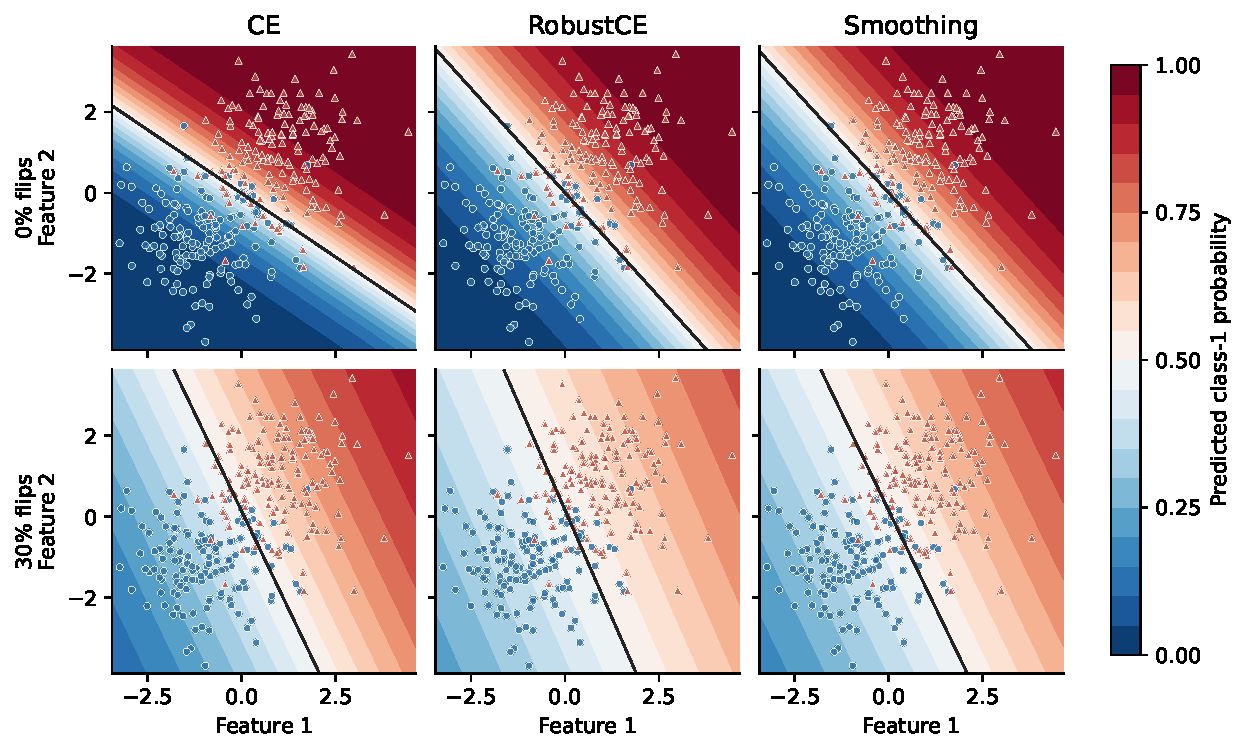
\includegraphics[width=\linewidth]{figures/gaussian.pdf}
\caption{Gaussian probability surfaces and $p_1=1/2$ contours for evaluation
seed 201. Markers show 300 clean test examples, circles for class 0 and
triangles for class 1. Rows differ in training-label flip probability.}
\label{fig:gaussian}
\end{figure}

\begin{figure}[p]
\centering
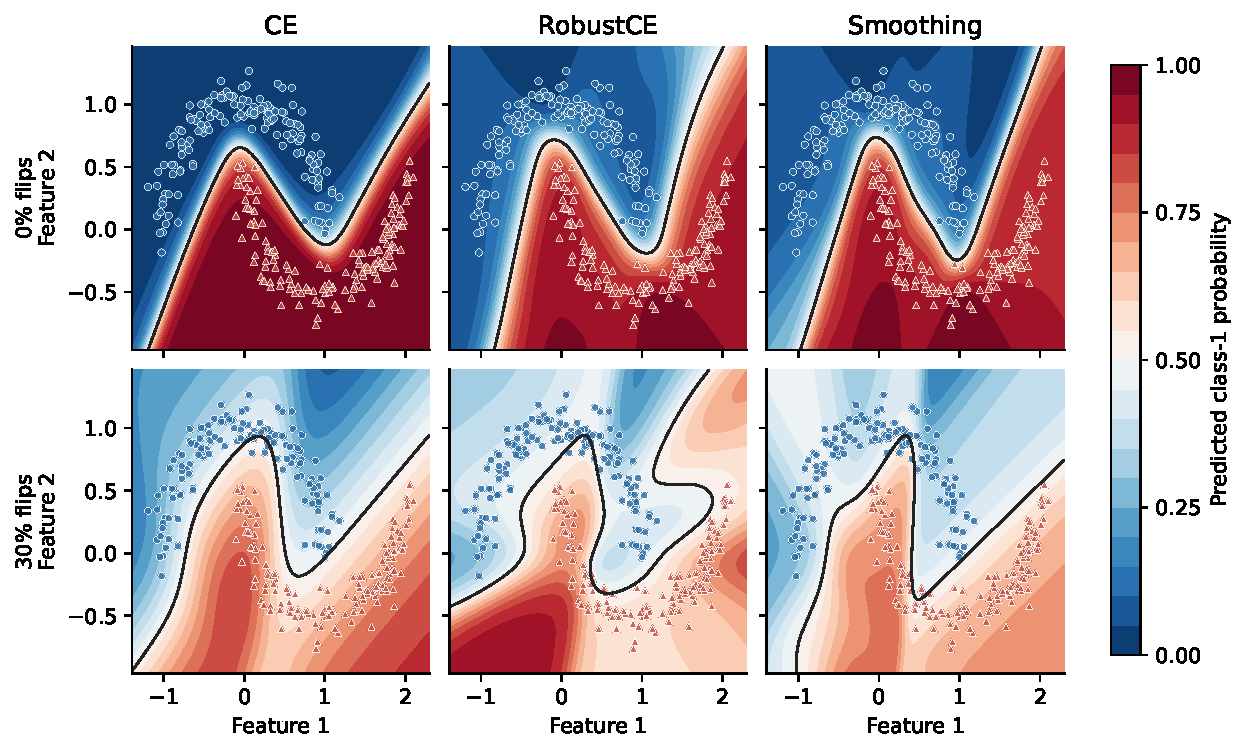
\includegraphics[width=\linewidth]{figures/semicircles.pdf}
\caption{Semicircle probability surfaces and $p_1=1/2$ contours for evaluation
seed 201. Marker and row conventions are as in Figure~\ref{fig:gaussian}.}
\label{fig:semicircles}
\end{figure}

\begin{figure}[p]
\centering
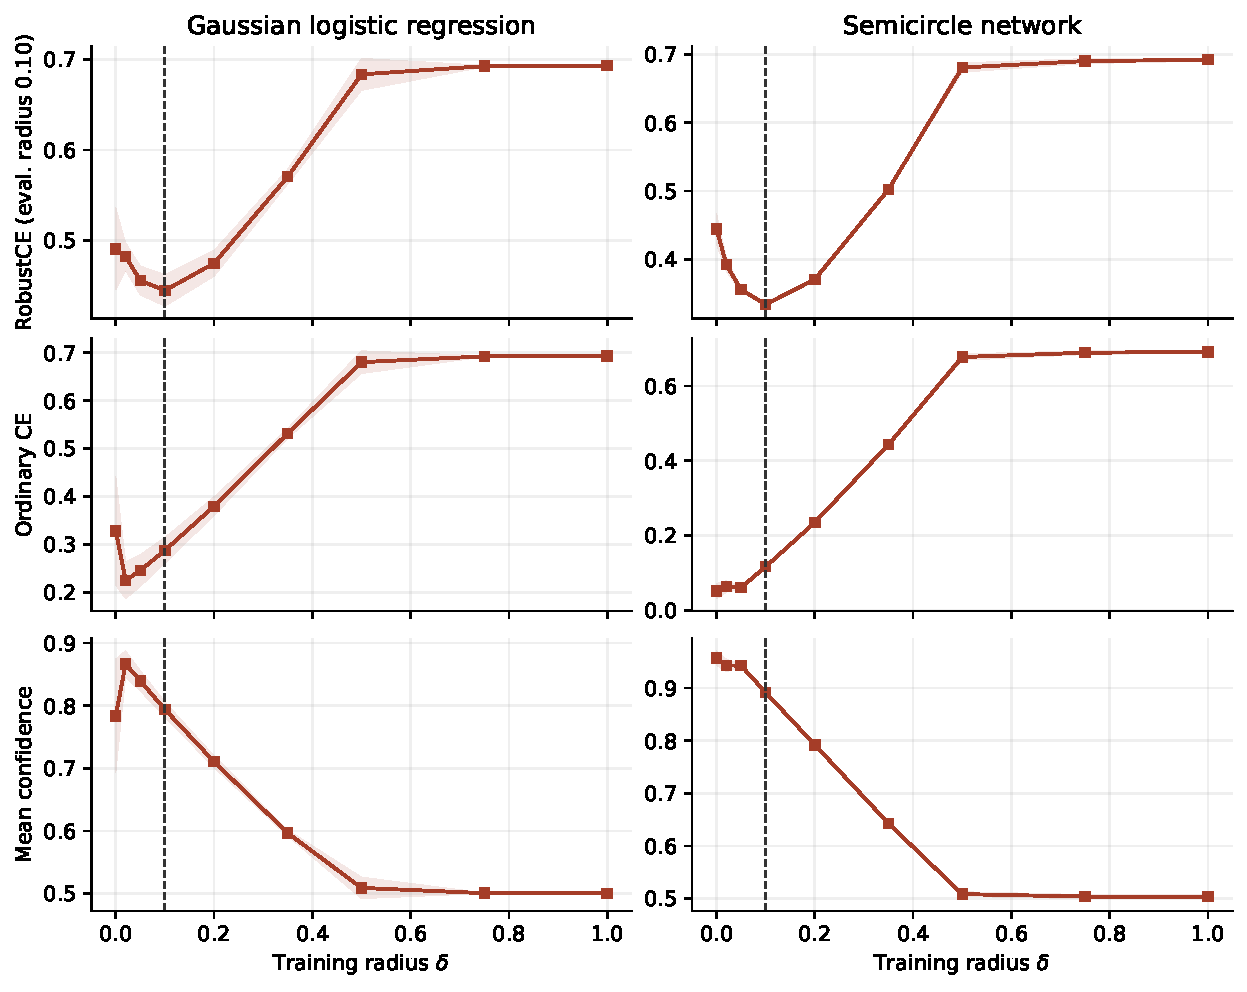
\includegraphics[width=\linewidth]{figures/radius.pdf}
\caption{Clean validation sensitivity across tuning seeds 101--105. At each
training radius the learning rate is selected by validation RobustCE at
$\delta_{\rm eval}=0.10$. Dashed lines indicate the selected radii. Bands
show one sample standard deviation.}
\label{fig:radius}
\end{figure}

\begin{figure}[p]
\centering
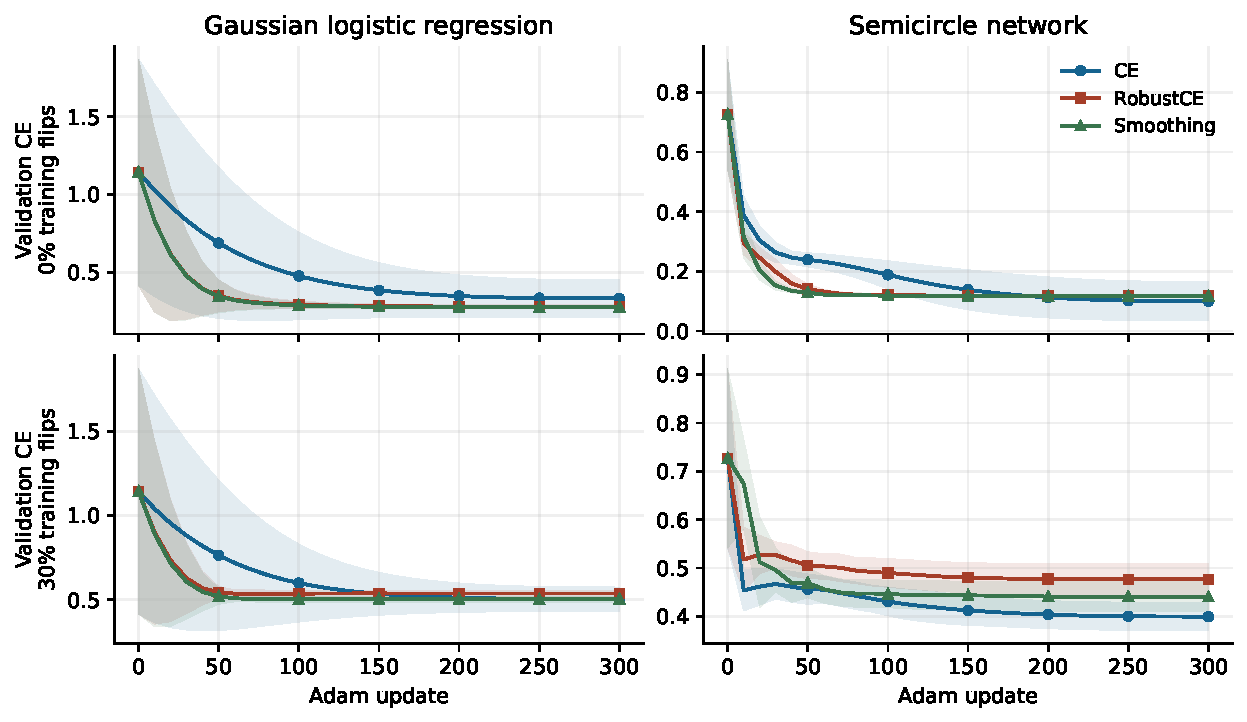
\includegraphics[width=\linewidth]{figures/learning.pdf}
\caption{Common clean validation CE during training with the frozen
settings, averaged across evaluation seeds 201--210. Bands show one sample
standard deviation.}
\label{fig:learning}
\end{figure}

\begin{figure}[p]
\centering
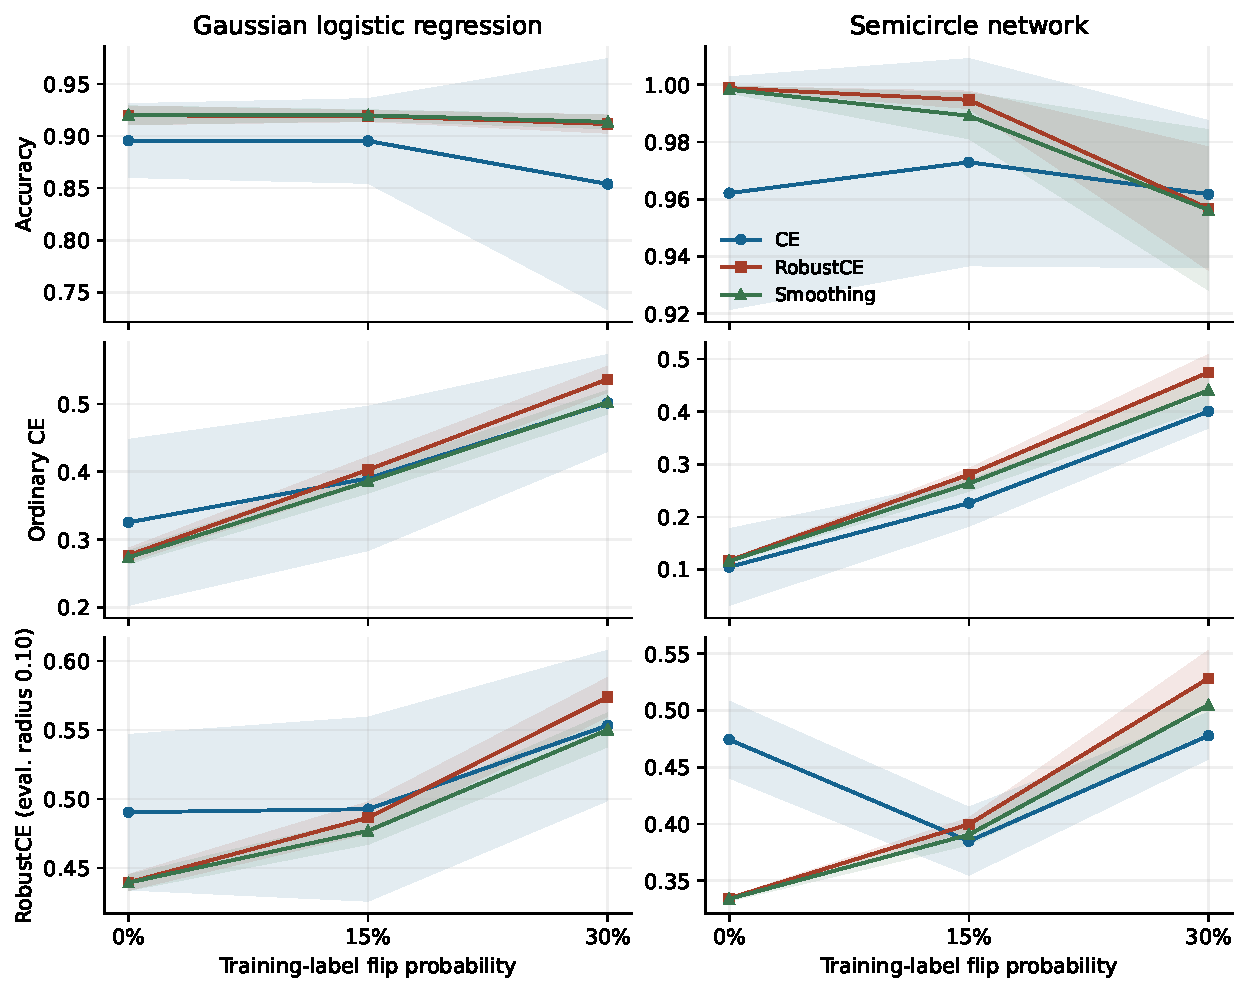
\includegraphics[width=\linewidth]{figures/corruption.pdf}
\caption{Clean held-out test performance versus training-label flip
probability across seeds 201--210. Bands show one sample standard
deviation. RobustCE is evaluated with radius $0.10$ throughout.}
\label{fig:corruption}
\end{figure}

\clearpage

\section{Critical analysis}
\subsection{Clean-label performance under the selected settings}
With clean training labels, RobustCE lowered common-radius test RobustCE
relative to CE by 0.051 for the Gaussian model and 0.140 for the semicircle
network. The mean accuracy differences were $+2.42$ and $+3.67$ percentage
points, respectively. The marginal paired intervals for these two metrics
excluded zero in both simulations. Ordinary test CE was less conclusive.
Its estimated change was $-0.048$ for the Gaussian model and $+0.012$ for
semicircles, with both intervals spanning zero.

The validation criterion matters for interpreting those differences. For
Gaussian CE, tuning selected rate 0.01, with mean validation CE 0.33.
Rates from 0.10 upward achieved ordinary validation CE near 0.21 while
increasing common-radius validation RobustCE from about 0.49 to 0.59.
For semicircles, increasing the CE learning rate from 0.03 to 0.10 likewise
lowered validation CE (about 0.05 to 0.01) while increasing validation RobustCE
(about 0.44 to 0.72). Tuning for the robust metric therefore rewarded some
incomplete optimization of ordinary CE under the fixed schedule. The
accuracy gains characterize these selected training pipelines. They leave
the comparison with fully optimized or CE-selected baselines open.

The two simulations completed 1,900 tuning fits and 180 evaluation fits
with zero numerical failures. The final learning rates were all interior
to the expanded grid. The selected $\delta$ and $\varepsilon$ were also
interior. Gaussian training took approximately 0.03--0.05 seconds per fit
and semicircle training approximately 0.10--0.13 seconds per fit when
summarized by condition means on the CPU used here.

\subsection{Radius and confidence}
Figure~\ref{fig:radius} shows the validation confidence approaching $1/2$
at large radii. This behavior follows from the hard-label objective.
Let $r$ be the conditional probability of an observed label 1 at a given
input. On the positive-logit branch the expected loss uses effective target
$r(1-\delta)$. On the negative-logit branch it uses effective target
$r+(1-r)\delta$. For $\delta\geq1/2$, the former is at most $1/2$ and the
latter is at least $1/2$, so a zero logit minimizes the conditional robust
risk at every input. At $\delta=1$ this follows directly from
$\operatorname{softplus}(|s|)$, independently of the labels. A nearly flat
probability surface can therefore retain an apparent threshold contour
while providing very little confidence or separation in the probabilities.

\subsection{Corruption and the smoothing comparison}
At 15\% flips, the paired intervals for common-radius RobustCE against CE
included zero in both datasets. The semicircle network had higher ordinary
test CE under RobustCE. At 30\% flips, semicircle RobustCE increased both
test losses relative to CE, by 0.074 for ordinary CE and 0.051 at the
common robust radius, with little evidence of a change in accuracy.
For Gaussians at 30\% flips, RobustCE had higher mean accuracy and higher
mean losses than CE, with wide paired intervals spanning zero. The mean
Gaussian confidence declined from 0.801 to 0.594 under RobustCE across
the clean and 30\% flip conditions.
Under independent symmetric flips, if the clean class-1 probability is $r_0$,
the observed probability is $\eta+(1-2\eta)r_0$. This already shrinks the
conditional probability toward $1/2$. For a high-confidence prediction
opposing a flipped label, RobustCE uses that flipped label as the worst-case
target, so the logit gradient is the full CE gradient against the prediction.
For a prediction agreeing with its observed label, RobustCE pushes the
probability toward $1/2$. These two effects explain why reducing extreme
confidence can help on clean labels and can aggravate underconfidence when
many labels are flipped.

With the selected $\varepsilon=0.20$ and $\delta=0.10$, the two methods
put the same mass on the alternative class for correctly signed logits.
Their gradients differ on incorrectly signed logits, which makes
smoothing a useful control for testing the value of the adaptive target.
The clean-label results for the two were close, especially for accuracy
and common-radius RobustCE. At 30\% flips, RobustCE was worse than
smoothing on both losses in both simulations, with paired intervals
excluding zero. At 15\% flips on semicircles, the adaptive loss gave a
small accuracy gain over smoothing ($0.56$ percentage points) while
raising both losses. Together these comparisons show a metric-dependent
trade-off and provide little evidence of a general advantage specific
to worst-case target selection.

\subsection{Limitations and follow-up}
The evidence is conditional on two balanced synthetic datasets, symmetric
flip noise, the fixed Adam budget, and one evaluation radius. Ten matched
seeds quantify variation in these settings, and the reported confidence
intervals remain sensitive to unusual runs. RobustCE is pointwise at least as
large as ordinary CE, so comparing the values of the different training
objectives cannot establish relative generalization. Common-radius robust
test CE measures worst-case log loss, while accuracy depends on the sign of
the logit and calibration depends on whether the probabilities agree with
observed frequencies.

A focused follow-up would repeat the matched sweep with a validation-fitted
scalar temperature for each method. Positive temperature scaling preserves
each model's decisions and changes its probabilities. Comparing paired
nominal CE, Brier score and reliability diagrams on a fresh clean test split
would show whether the differences in probability quality can be explained
by global confidence shrinkage. A consistent residual advantage of RobustCE
over confidence-matched smoothing on a prespecified metric would provide
stronger evidence for the adaptive target mechanism.

\end{document}
